\documentclass{article}
\usepackage{graphicx}
\graphicspath{ {images/} }

\title{The Book of Special Relativity}
\date{May 17th, 2017}
\author{Sishaar Rao}

\begin{document}
\pagenumbering{gobble}
\maketitle
\newpage
\pagenumbering{arabic}

Special relativity is a theory proposed by Albert Einstein that describes the propagation of matter and light at high speeds. It was invented to explain the observed behavior of electric and magnetic fields, which it beautifully reconciles into a single so-called electromagnetic field, and also to resolve a number of paradoxes that arise when considering travel at large speeds. Special relativity also explains the behavior of fast-traveling particle, including the fact that fast-traveling unstable particles appear to decay slower than identical particles traveling slower. Special relativity is an indispensable tool of modern physics, and its predictions have been experimentally tested time and time again without any discrepancies turning up. Special relativity reduces to Newtonian mechanics in the limit of small speeds.

\vspace{5mm}

According to special relativity, no wave or particle may travel at a speed greater than the speed of light c. Therefore, the usual rules from Newtonian mechanics do not apply when adding velocities that are large enough. For example, if a particle travels at a speed \( v \) with respect to a stationary observer, and another particle travels at a speed \( v' \)  with respect to the first particle, the speed \( u \) of particle two seen by the observer is not  as would be the case in Newtonian mechanics, but rather
\[
  u = \frac{v + v'}{1 + \frac{vv'}{c^2}}
\]

\newpage
\section{Invariance of Length’s Measured Perpendicular to Relative Motion}

\begin{figure}[!htb]
  \centering
  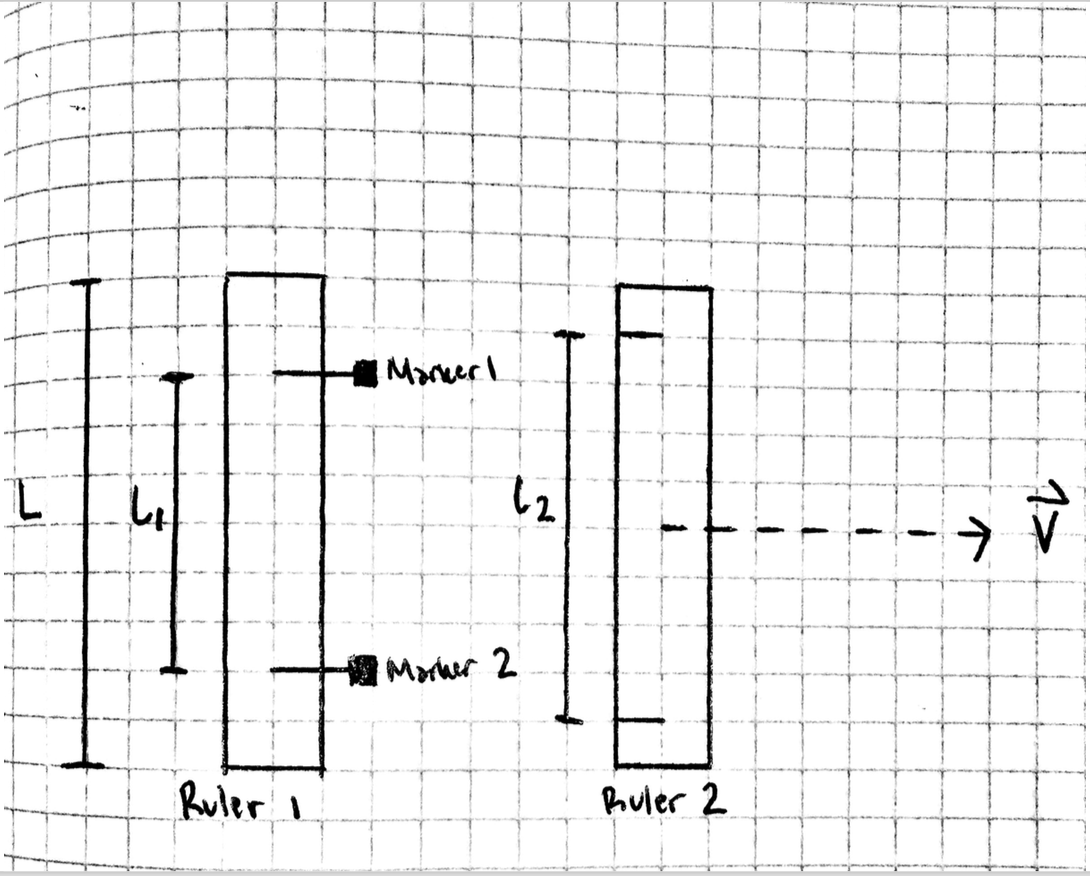
\includegraphics[width=100mm]{sticks}\par
  \caption{Two rulers perpendicularly flying past eachother}
\end{figure}

In the figure above, we are presented with a thought experiment:

\vspace{2mm}

Suppose we are given two rulers, Ruler 1 and Ruler 2 of length \(L\). Ruler 1 has two markers attached on it with a separation of \(L_1\). Our hypothesis is that if Ruler 2 is flying perpendicularly by Ruler 1 with a speed \(\vec{v}\), then Ruler 2 will become shorter than Ruler 1.

If indeed Ruler 2 does become shorter, then as it travels by Ruler 1, the tick marks drawn by the marker on Ruler 1 will not have a separation of \(L_1\) but rather of \(L_2\) where \(L_2 > L_1\). However, according to the principle of relativity it is equally valid to think of Ruler 2 as stationary and Ruler 1 as moving during the flyby. From this perspective, the moving Ruler (now Ruler 1) is \textit{longer} than the stationary stick, as that is the only way for \(L_2 > L_1\) to be true. Thus, our hypothesis that our moving Ruler will become shorter faces a contradition, and is \textbf{rejected}.

\vspace{2mm}

We can thus conclude: \textit{
  A stick moving perpendicular to its length has the same length as an identical stick that is stationary.
}

\newpage
\section{Time Dilation}

\begin{figure}[!htb]
  \centering
  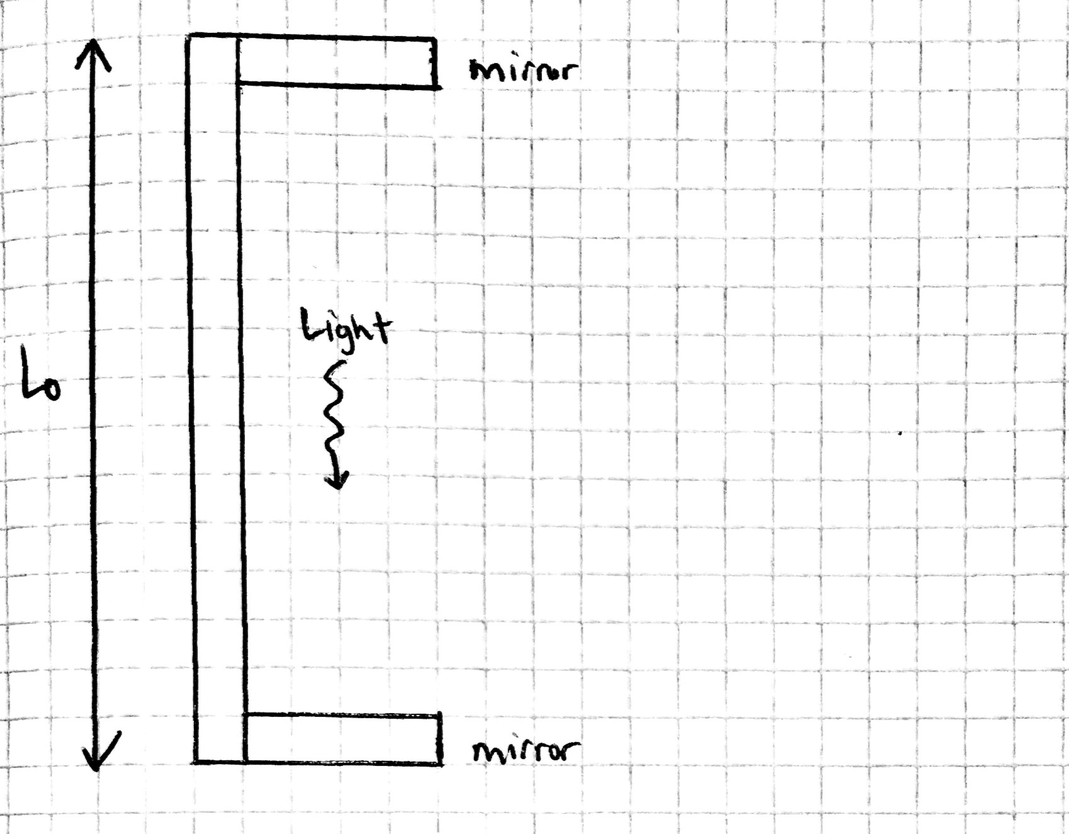
\includegraphics[width=100mm]{lightclock}\par
  \caption{Light Clock}
\end{figure}

\begin{figure}[!htb]
  \centering
  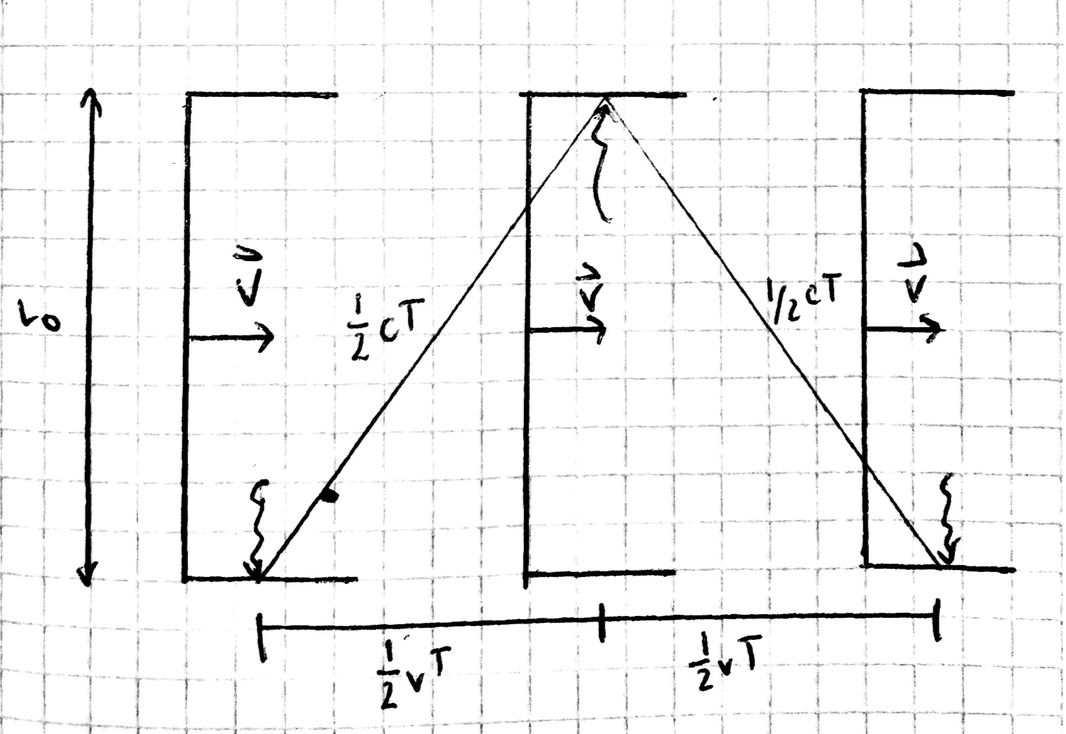
\includegraphics[width=100mm]{lightclockmoving}\par
  \caption{A Light Clock Moving with Velocity \(\vec{v}\)}
\end{figure}

\newpage
Suppose we construct a Light Clock, which is defined as the structure in Figure 1. The time between ticks \(T_0\) on a light clock is the time between when the light hits, say the lower mirror. Since the light travels a length \(L_0\), we can relate the time between ticks by \(2L_0 = cT_0\).

Consider when the light clock is moving at a velocity \(\vec(v)\). In this frame of reference, the clock moves a distance \(vT_0\) in between ticks, as demonstrated in Figure 2. Thus, the distance that the light is travelling by the Pythagorean theorem is now expressed as
\[
cT_0 = 2\sqrt{L_0^2 + (\frac{1}{2}vT_0)^2}
\]

But since we know that the speed of light is the same in all inertial frames, we can substitute in \(L_0 = \frac{1}{2}cT_0\) and you get
\[
cT = 2\sqrt{(\frac{1}{2}cT_0)^2 + (\frac{1}{2}vT)^2}
\]

Solving for T yields
\[
  T = \frac{T_0}{\sqrt{1 - (\frac{\vec{v}^2}{c^2})}}
\]

Since we know that \(\vec{v} < c\), we can deduce from the given equation that the time T between ticks in a reference frame moving with velocity \(\vec(v)\) is greater than time \(T_0\) between ticks in the proper reference frame of the clocks.

This brings us to question: Does this fact only hold true for light clocks or all clocks in general? It turns out that the answer is yes. Consider the following thought experiment:

In the proper reference frame of the clocks, the time between ticks of both clocks is exactly one second. A light-sensitive film is placed on the face of the conventional clock, behind a rotating disk. Each time the light pulse reflects off the lower mirror, a narrow region of the light-sensitive paper directly behind the slot gets exposed. These exposed regions will be aligned with the tick marks, and all observers must agree with this permanent record.

In the reference frame where the clocks are both moving, the light pulse exposes the film behind the slot on the clock face each time the pulse reflects off the lower mirror. Because the light clock is moving, the time between these reflections is greater than 1 s, in accordance with equation for T. When an observer of original reference frame sees that the lines appearing where the film was exposed are aligned with the tick marks, they realize that in their reference frame the conventional clock runs slow in exactly the same manner that the light clock runs slow and that this has nothing to do with the mechanism of the conventional clock. Thus, we conclude that all moving clocks run slow in exactly the same manner that a moving light clock runs slow. Because this is the case, we conclude that it is time itself that runs slow. We call this phenomena \textbf{Time Dilation}.

\newpage
\section{Length Contraction}

Earlier, we demonstrated that the length of a stick moving perpendicular to its length and the length of an identical stationary stick are equal. However, the key takeaway from this is that this only applies when the stick is perpendicular. Here, we analyze what happens when we analyze a situation where a stick is moving parallel to its length.

Suppose we are given a Light Clock in two scenarios as demonstrated by the figures below.
\begin{figure}[!htb]
  \centering
  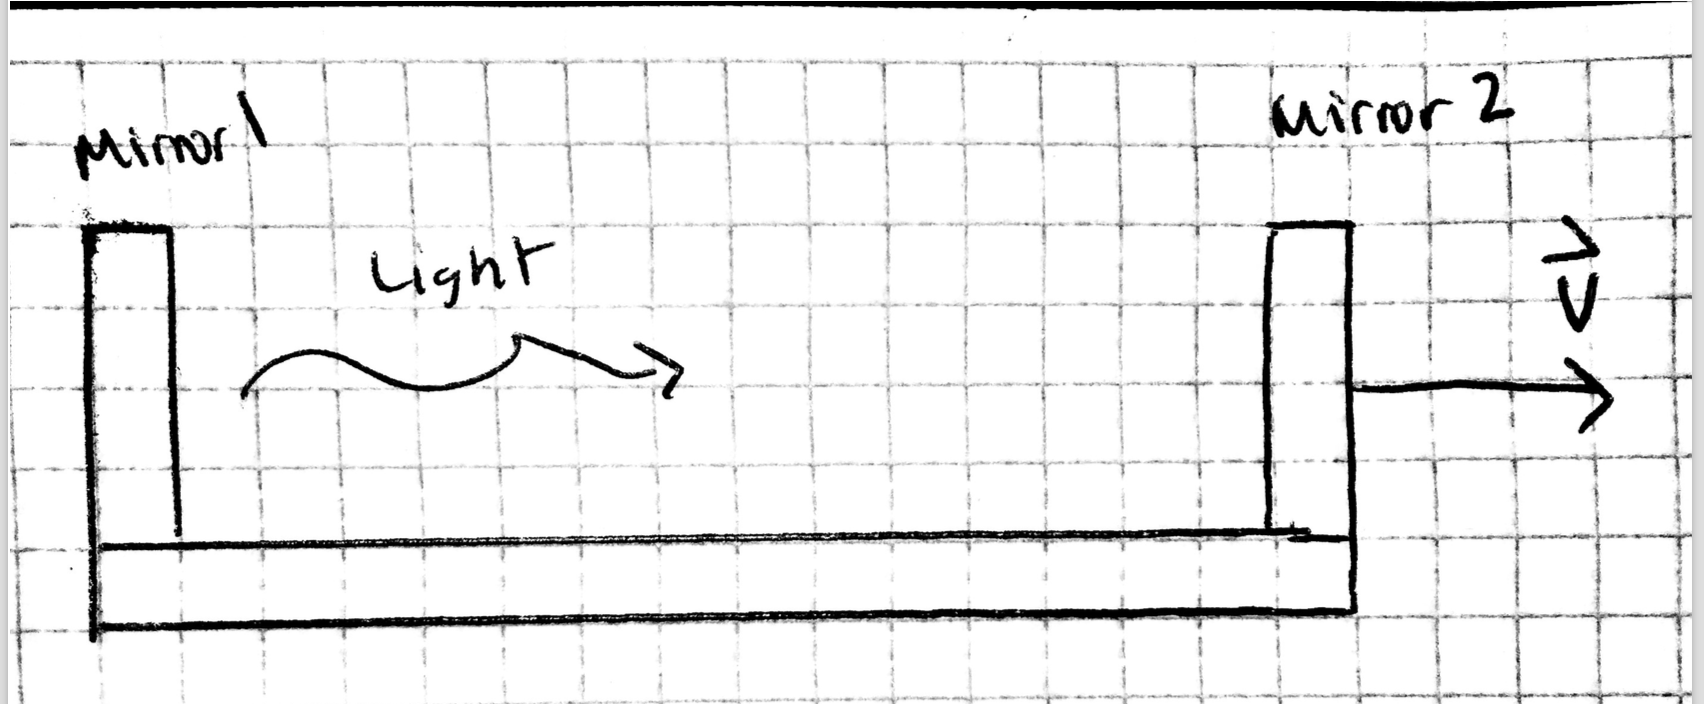
\includegraphics[width=100mm]{lengthcontraction1}\par
  \caption{Light Clock travelling Parallel to Length}
\end{figure}

Suppose the Light Clock has length \(L_0\). Thus, the time \(T_0\) between ticks of the light clock when \(\vec(v) = 0\) is \(\frac{2L_0}{c}\)

However, if  \(\vec(v) \neq 0\) then the light has to travel a greater distance to hit the right side and a shorter distance to come back and hit the left side. The distance travelled by the light in stationary reference frame is \(cT_0\).

When the box is not stationary, let us define three events:\newline
Event 0: Light pulse reflects off the mirror at the left end.\newline
Event 1: Light pulse reflects off the mirror at the right end.\newline
Event 2: Light pulse reflects off at the mirror at the left end.\newline

The times of occurences of these events are labeled \(t_0 t_1 t_2\). In the time between events 0 and 1, the clock moves a distance \(\vec{v}(t_1 - t_0)\) and the light pulse travels a distance \(c(t_1 - t_0)\). We can express this as
\[
  c(t_1 - t_0) = L + v(t_1 - t_0)
\]

Similarly for the time between events 1 and 2, we can express it as
\[
  c(t_2 - t_1) = L + v(t_2 - t_1)
\]

Using substitution to elimate \(t_1\), we can now express this as
\[
  t_2 - t_0 = \frac{\frac{2L}{c}}{1 - \frac{\vec{v}^2}{c^2}}
\]

Employing our Time Dilation equation to Events 0 and 2, we can state that
\[
  t_2 - t_0 = \frac{\frac{2L_0}{c}}{\sqrt{1 - \frac{\vec{v}^2}{c^2}}}
\]

By setting these equations equal to eachother and solving for L, we get that

\[
  L = L_0\sqrt{1 - \frac{\vec{v}^2}{c^2}}
\]

Note that this formula does not involve any properties of the stick but rather properties of space and time. 

\newpage
\section{Desynchronization}
Suppose we are given two clocks, as demonstrated in the figure below.
\begin{figure}[!htb]
  \centering
  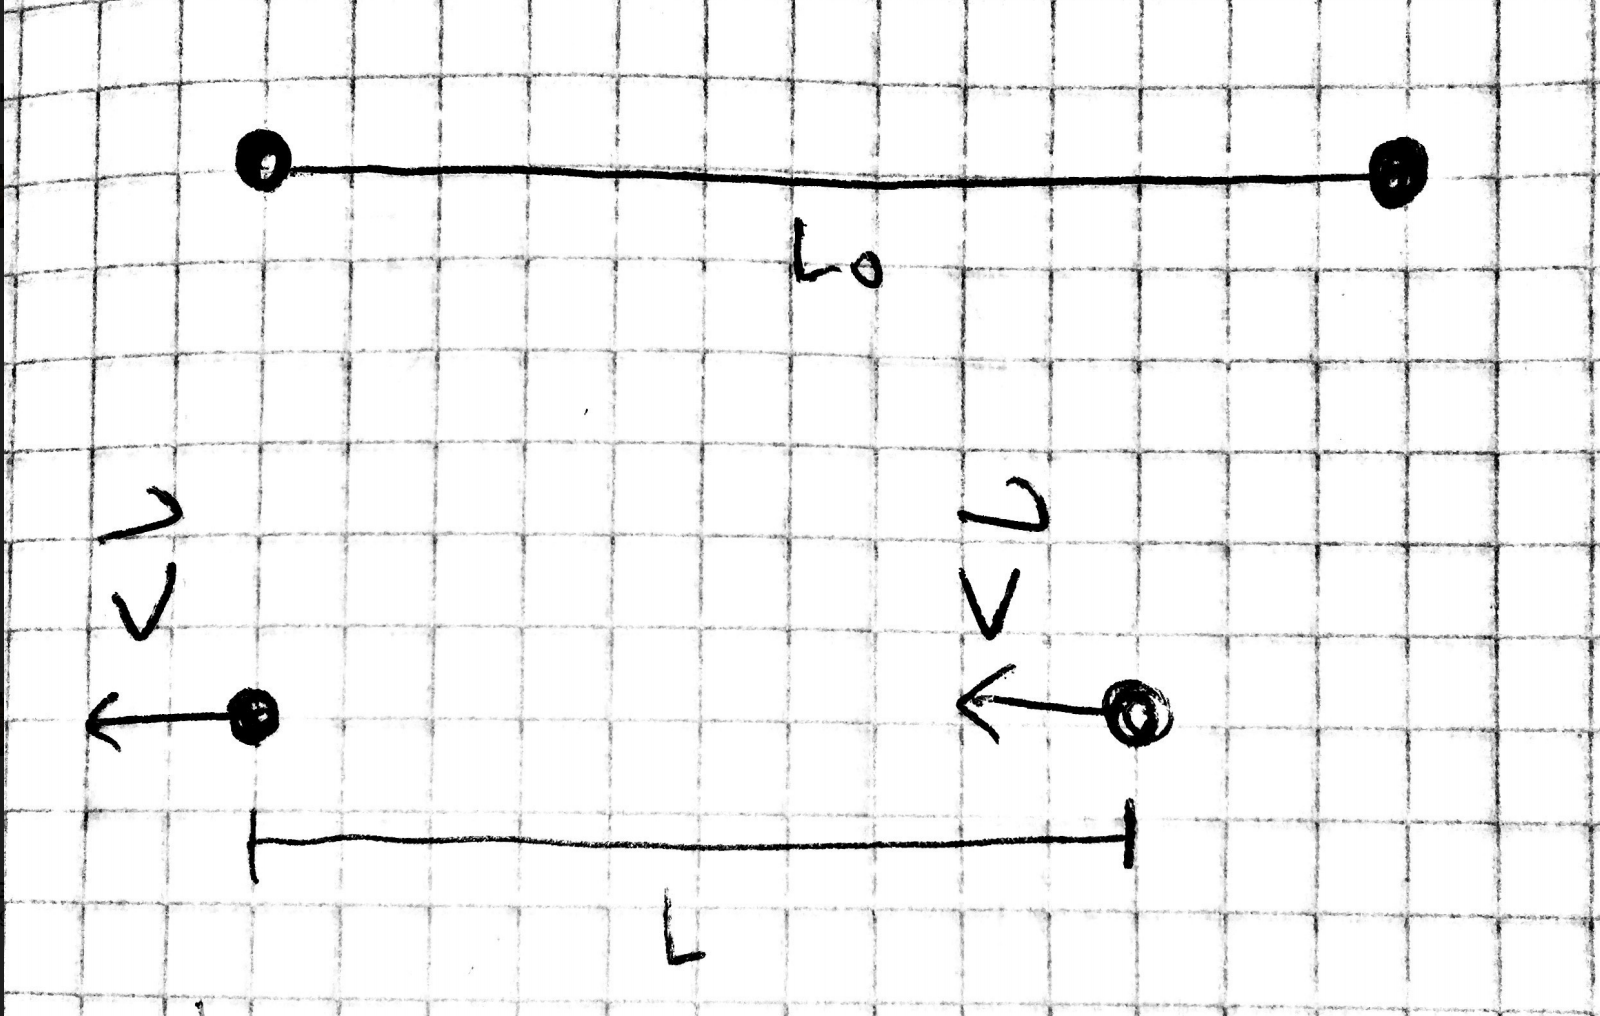
\includegraphics[width=100mm]{desync1}\par
  \caption{Two clocks in different reference planes}
\end{figure}

In the top frame, the two clocks are at rest relative to eachother, separated by a distance \(L_0\).

To synchronize these clocks there is a flashlamp on clock A (the left-hand clock) and a light-sensitive film on the face of clock B (the right-hand clock). The alarm on clock A is set to energize the flashlamp when the second hand on clock A passes zero. Like the conventional clock described previously, clock B has only a second hand, a rotating opaque disk with a slot to indicate the time. Behind the disk is a light-sensitive film. When the light from the flash reaches clock B, the film is illuminated on the narrow region behind the slot. This provides a lasting record of the reading on clock B when the light from the flashlamp reaches it. Let this reading be \(t_1\)

In the rest frame of the clocks, the time for the light to travel at speed c from clock A
to clock B is \(\frac{L_0}{c}\), so when the light arrives at clock B, clock A 0
reads  \(\frac{L_0}{c}\) and clock B reads \(t_1\). To synchronize the two clocks, we turn Clock B back by \(\Delta t = t_1 - \frac{L_0}{c}\). We now want to determine whether or not this synchronization holds in a reference frame moving with velocity \(\vec(v)\).

In frame 2 (the bottom frame) we know that the distance L from before is
\[
  L = L_0\sqrt{1 - \frac{\vec{v}^2}{c^2}}
\]
where Clock B is moving towards the flashlamp. In this frame, the light traveling from clock A to clock B travels a distance \(L - \vec{v}t\), where \(t\) is the time required for the light to travel the distance. We can equate this as \(ct = L - vt\). Solving for t gives us \(t = \frac{L}{c + \vec{v}}\)

During time \(t\) the readings on both clocks advance not by t but by \(t\sqrt{1 - \frac{\vec{v}^2}{c^2}}\) where \(t = \frac{L}{c + \vec{v}}\).

Substituting and simplifying gives us
\[
  \frac{L_0}{c} - \frac{vL_0}{c^2}
\]

Thus, when the light arrives at clock B, clock B reads \(\frac{L_0}{c}\) and clock A reads \(\frac{L_0}{c} - \frac{vL_0}{c^2}\). Therefore, in frame 2, clock B is ahead of clock A by \(\frac{vL_0}{c^2}\).


We can summarize this as:\newline
If two clocks that are moving with the same velocity are synchronized in their rest frame, then in a frame where they move with speed v parallel to the line joining them, the clock in the rear is ahead of the clock in front by \(\frac{vL_0}{c^2}\)

This desyncrhonization between clocks A and B can be summarized with formulas
\[
  \Delta t_b = \frac{L_a \frac{\vec{v}^2}{c^2}}{\sqrt{1 - \frac{\vec{v}^2}{c^2}}}
\]
\newpage
\section{Synthesis of Lorentz Transformation}


\end{document}
